% headers
\documentclass[12pt, a4paper]{report}
\usepackage[utf8]{inputenc}
\usepackage{graphicx}
\usepackage{amsmath}
\graphicspath{{images/}}
\title{First document: Hello Latex}
\author{Pei-Lun Hsu}
\date{\today}



% body start
\begin{document}

% title
\maketitle

% Abstracts
\begin{abstract}
    This is a simple paragraph at the beginning of the document. A brief introduction about the main subject.
\end{abstract}

\tableofcontents

% new Chapter
\chapter{First Chapter}
This some paragraph after the abstract. This some paragraph after the abstract. This some paragraph after the abstract. This some paragraph after the abstract. This some paragraph after the abstract.

\section{Problems}
This is the first section.

Lorem ipsum dolor sit amet, consectetur adipiscing elit, sed do eiusmod tempor incididunt ut labore et dolore magna aliqua. Ut enim ad minim veniam, quis nostrud exercitation ullamco laboris nisi ut aliquip ex ea commodo consequat. Duis aute irure dolor in reprehenderit in voluptate velit esse cillum dolore eu fugiat nulla pariatur. Excepteur sint occaecat cupidatat non proident, sunt in culpa qui officia deserunt mollit anim id est laborum.

\section{Goals and Purposed}
This is the second section.

Lorem ipsum dolor sit amet, consectetur adipiscing elit, sed do eiusmod tempor incididunt ut labore et dolore magna aliqua. Ut enim ad minim veniam, quis nostrud exercitation ullamco laboris nisi ut aliquip ex ea commodo consequat. Duis aute irure dolor in reprehenderit in voluptate velit esse cillum dolore eu fugiat nulla pariatur. Excepteur sint occaecat cupidatat non proident, sunt in culpa qui officia deserunt mollit anim id est laborum.

\subsection{Purpose 1}
Lorem ipsum dolor sit amet, consectetur adipiscing elit, sed do eiusmod tempor incididunt ut labore.

\begin{table}
    \centering
    \begin{tabular}{c|c|c}
    \hline
    cell1 & cell2 & cell3 \\
    cell4 & cell5 & cell6 \\
    cell7 & cell8 & cell9 \\
    \hline
    \end{tabular}
    \caption{Caption of the figure1}
    \label{tab:my_label}
\end{table}


Table \ref{tab:double sep} is an example of the table with double separation line.
\begin{table}[h]
    \centering
    \begin{tabular}{||c c c||}
    \hline
    col1 & col2 & col3\\[0.5ex]
    \hline \hline
    4 & 5 & 8 \\
    \hline
    3 & 0 & 30 \\
    \hline
    7 & 23 & 39 \\
    \hline
    92 & 9 & 20 \\ [1ex]
    \hline
    \end{tabular}
    \caption{figure caption 2}
    \label{tab:double sep}
\end{table}

\subsection{Purpose 2}
Lorem ipsum dolor sit amet, consectetur adipiscing elit, sed do eiusmod tempor incididunt ut labore.

% section without the numbering
\section*{Others}
\addcontentsline{toc}{section}{Others}
Lorem ipsum dolor sit amet, consectetur adipiscing elit, sed do eiusmod tempor incididunt ut labore.

\marginpar{The new section start point will be pointed out 
by an arrow}

% % Add contents after the title and the author
% First document. This is a simple example, with no extra parameters or packages included. Add more sentences.

% % bold italics and underlining font
% Show some words in \textbf{the bold font.}
% Show some words in \textit{the italic font.}
% Show some words with \underline{the \textbf{underline}s.}

% % add image
% \begin{figure}[h]
%     \centering
%     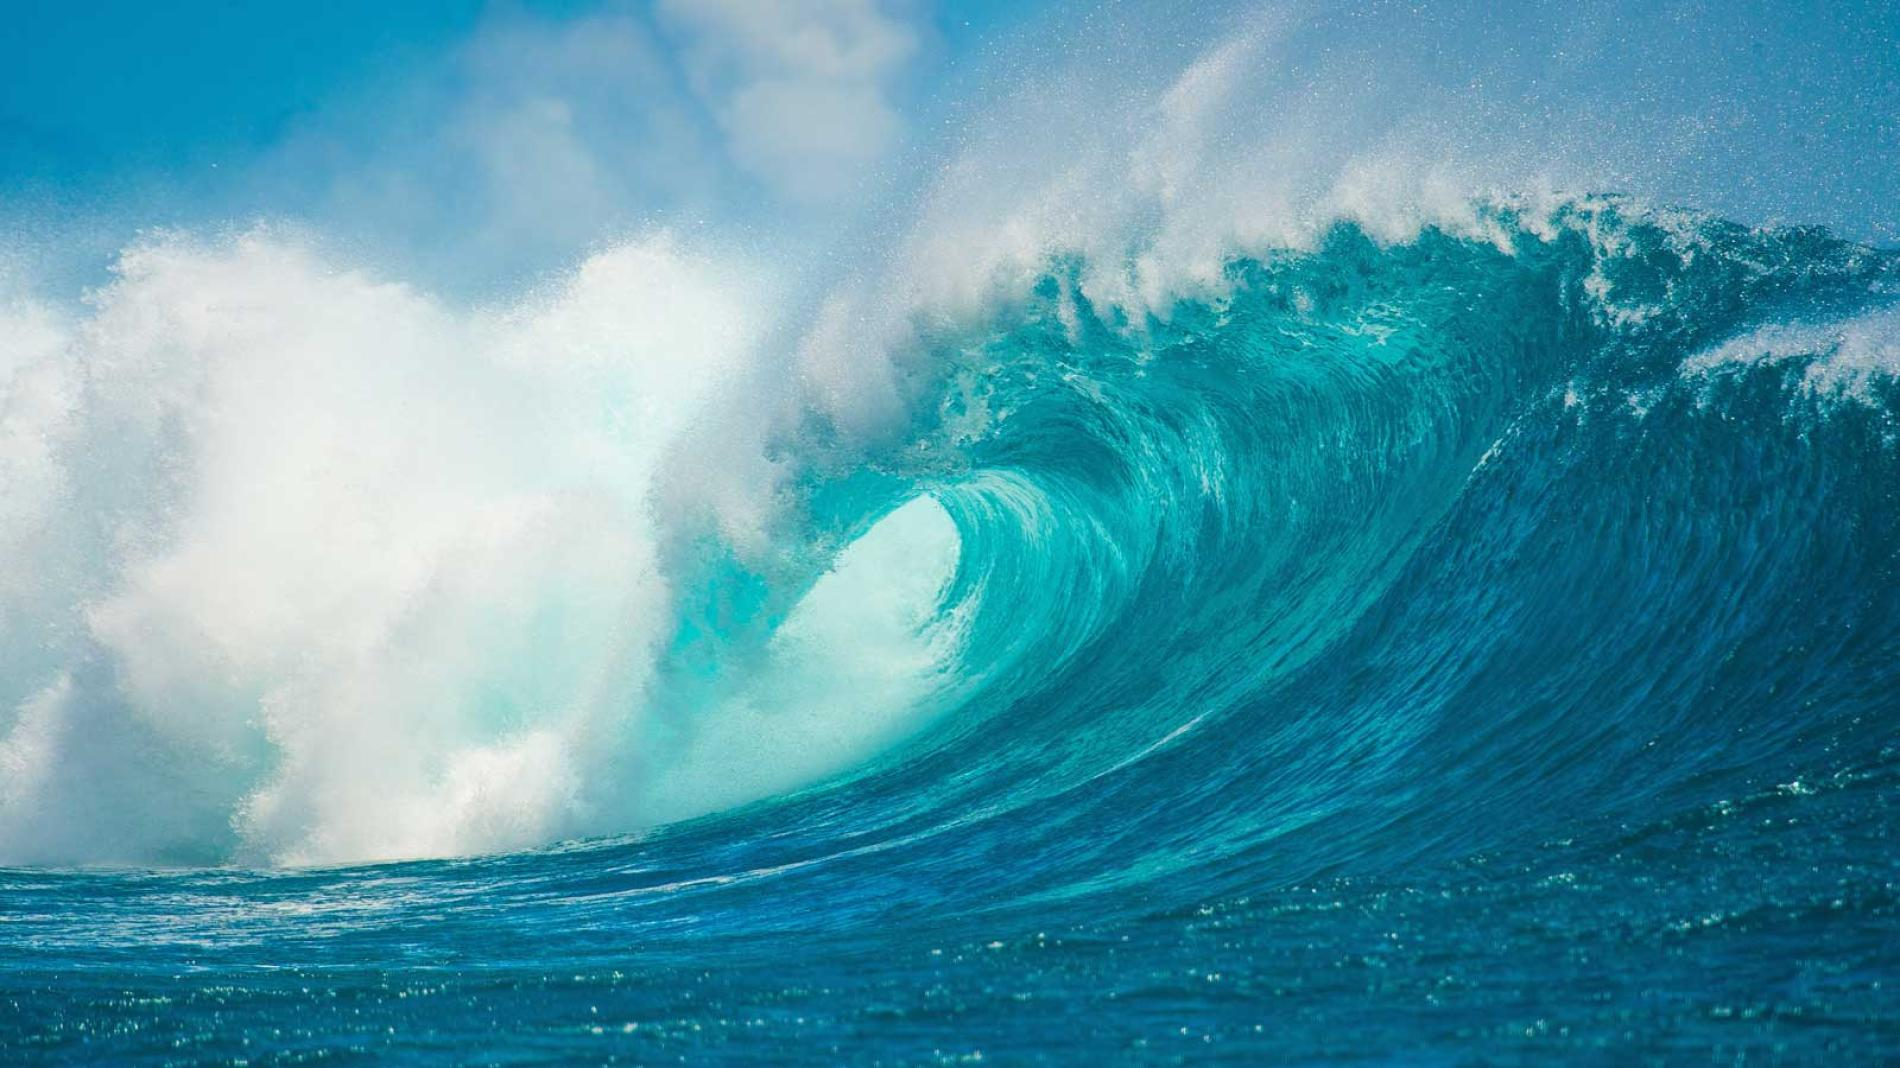
\includegraphics[width=0.5\textwidth]{test2}
%     \caption{A example figure}
%     \label{fig:my_label}
% \end{figure}
% As you can see in the figure \ref{fig:my_label}, the performance of the time-dependent neural network is better.

% % Creating lists
% % 1. unordered lists
% \begin{itemize}
%     \item clock
%     \item boot
%     \item flower
% \end{itemize}
% % 2. order list
% \begin{enumerate}
%     \item jimmy rank first
%     \item Jenny ranks second
%     \item Mars ranks third
% \end{enumerate}

% % math inline mode
% In physics, the mass-energy equivalence is stated by the equation $E=mc^2$, discovered in 1905 by Einstein.
% % math display model
% % unnumbered
% The mass-energy equation
% \begin{equation}
% E=mc^2 
% \end{equation} 
% In natural unit ($c=1$), the formula express the identity 
% \begin{equation}
% E=m
% \end{equation}

% % operator are prefixed with a backslash
% Some equation with complex operators
% \begin{equation}
% \sin(\omega)
% \end{equation}



\end{document}

